\label{sec:algorithms}
\begin{algorithm}[!ht]
	\SetArgSty{}
	\SetKwProg{Proc}{}{ :}{}
	\KwIn{Subspace dimension $s = 2p$,\newline
				 $V_1 \in \mathbb{R}^{n \times s}$ with rank $s$,\newline
				 $A = A^T; B$ is symmetric positive definite
	}
	\KwOut{The smallest $p$ eigenvalues ($\Theta_k$) and their corresponding eigenvectors ($Y_k$)}
	\For{$k = 1 \rightarrow$ mat\_iter}{
		\Proc{$B$-orthonormalize $V_k \rightarrow Z_k$}{
			Compute $\hat{B}_k = BV_k$\;\nllabel{ln:B}
			Compute all eigenpairs of $V_k^T B V_k$, $V_k^T \hat{B}_k = \Upsilon_k \Sigma_k \Upsilon_k^T$\;
			Compute $Z_k = V_k \Upsilon_k \Sigma_k^{-1/2}$\;
			Compute $\dot{B}_k = \hat{B}_k \Upsilon_k \Sigma_k^{-1/2}$\;\nllabel{ln:Bdot}
		}
		\Proc{Perform the Rayleigh-Ritz procedure to obtain the Ritz eigenpairs ($AY_k \approx BY_k\Theta_k$)}{
			Compute $\hat{A}_k = AZ_k$\;\nllabel{ln:A}
			Compute all eigenpairs of $Z_k^T A Z_k$, $Z_k^T \hat{A}_k = \Pi_k \Theta_k \Pi_k^T$\;
			Sort the eigenpairs ($\Theta_k, \Pi_k$) in assending order of $\Theta_k$\;
			Compute the Ritz vectors $Y_k = Z_k \Pi_k$\;
			Compute $\ddot{B}_k = \dot{B}_k \Pi_k$\;\nllabel{ln:Bddot}
			Compute $\dot{A}_k = \hat{A}_k \Pi_k$\;\nllabel{ln:Adot}
		}
		Compute the first $p$ columns of the residual vectors $\Phi_k = \dot{A} - \ddot{B}\Theta_k$\;\nllabel{ln:phi}
		\Proc{Test for convergence}{
			\lIf{$\|\Phi_k e_j\|_2 / \theta_j \le \tau; \forall j \le p$}{\KwSty{break}}
		}
		\Proc{Solve the reduced system $P_k A \Delta_k = P_k A Y_k$ where $P_k = I - B Y_k \left(Y_k^T B^2 Y_k\right)^{-1}Y_k^T B$}{
			Compute the QR decomposition of $BY_k$, $\ddot{B}_k = \left[Q_{k1}\ Q_{k2}\right]\left[R_k^T\ 0\right]^T$\;
			Compute $N_k = P_k \dot{A}_k Y_k$\;
			Use iterative solver to solve $P_k A \Delta_k = N_k$ with initial guess $\Delta_k = 0$\;
		}
		Compute $V_{k+1} = Y_k - \Delta_k$\;
	}
	\caption{Basic Trace Minimization}\label{alg:basic}
\end{algorithm}
The trace minimization algorithm is motivated by the following theorem.
\begin{theorem}[Sameh and Wisniewski\cite{sameh1982}]
	Let $A$ and $B$ be as given in problem \ref{eq:eig}; and let $X*$ be the set of all $n \times p$ matrices $X$ for
	which $X^T B X = I_p, 1 \le p \le n$. Then
	\begin{equation}
		\min_{X \in X*} tr(X^T A X) = \sum_{i=1}^p \lambda_i,
	\end{equation}
	wher $\lambda_1 \le \lambda_2 \le \cdots \le \lambda_n$ are the eigenvalues of problem \ref{eq:eig}. The equality
	holds if and only if the columns of the matrix $X$, which achieves the minimum, span the eigenspace corresponding
	to the smallest $p$ eigenvalues.
\end{theorem}
Hence, if we could find such $X$ that minimizes the trace, we would obtain the smallest $p$ eigenpairs. In the
trace minimization algorithm, we start with a random $X$ in the subspace and iteratively refine it by computing a
correction term $\Delta$ until the trace is minimized, i.e. in each iteration,
\begin{equation}
	tr\left((Y - \Delta)^T A (Y - \Delta)\right) < tr\left(Y^T A Y\right).
\end{equation}
To achieve the convergence, we define the function
\begin{align}
	\phi(\Delta) &= tr\left((Y - \Delta)^T A (Y - \Delta)\right) - tr\left(Y^T A Y\right)\nonumber\\
							 &= 2tr\left(Y^T A\Delta\right) - tr(\Delta^T A\Delta),
\end{align}
and seek to maximize $\phi$ subject to $Y^T B \Delta = 0$. This can be done by taking the derivates of the function
\begin{equation}
	\psi(\Delta, \mathcal{L}) = 2tr\left(Y^T A\Delta\right) - tr(\Delta^T A\Delta) - tr(\mathcal{L}\cdot Y^T B\Delta),
\end{equation}
where $\mathcal{L}$ is a Langrange multiplier, with respect to $\Delta$ and $\mathcal{L}$ and set them to $0$. This
would yield the following two equations.
\begin{align}
	\frac{\partial \psi}{\partial \Delta} &= 0 &\Rightarrow &&2AY - 2A\Delta - BY\mathcal{L}^T &= 0,\text{ and}\\
	\frac{\partial \psi}{\partial \mathcal{L}} &= 0 &\Rightarrow &&Y^T B\Delta &= 0,
\end{align}
which can be expressed as a saddle-point equation,
\begin{equation}
	\begin{bmatrix}
		A & BY\\
		Y^T B & 0
	\end{bmatrix} \begin{bmatrix}
		\Delta \\ L
	\end{bmatrix} = \begin{bmatrix}
		AY \\ 0
	\end{bmatrix}.
\end{equation}
This saddle-point equation is further reduced to the following system in \cite{sameh1982}.
\begin{equation}
	PA\Delta = PAY,
\end{equation}
where $P = I - BY(Y^T B^2 Y)^{-1} Y^T B$, on which our project implementation is based.

\subsection{Basic Trace Minimization Algorithm}
The basic trace minimization algorithm is outlined in Algorithm~\ref{alg:basic}. Note that since both $A$ and $B$ are
large, we reduce the number of multiplications involving $A$ and $B$ to one each (Lines~\ref{ln:B} and~\ref{ln:A})
except within the iterative solver. This is achieved by postmultiplying the products $BV_k$ and $AZ_k$ by other
matrices (Lines~\ref{ln:Bdot},~\ref{ln:Bddot} and~\ref{ln:Adot}). In addition, we only compute the first $p$ columns
of the residual matrix $\Phi$ (Line~\ref{ln:phi}) since we only need the first $p$ columns to converge.

\subsection{Trace Minimization Algorithm with Deflation}
\begin{figure}[h]
	\centering
	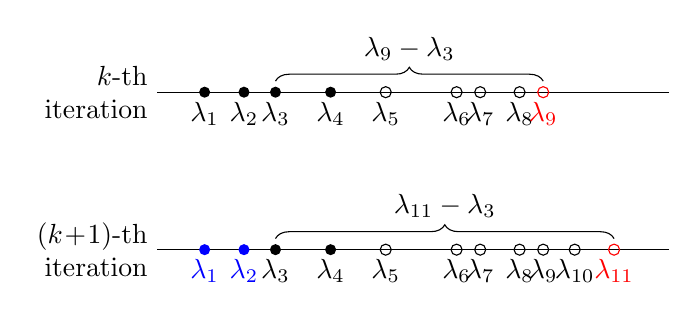
\begin{tikzpicture}
		\draw (7, 1) -- (0.5, 1) node[left, text width=40pt, align=right] {$k$-th\\ iteration};
		\draw (7, -1) -- (0.5, -1) node[left, text width=40pt, align=right] {$(k+1)$-th\\ iteration};
		\draw[decorate, decoration={brace, amplitude=5pt}, yshift=4pt] (2.0, 1) -- (5.4, 1)
			node[midway, above, yshift=4pt] {$\lambda_9 - \lambda_3$};
		\draw[decorate, decoration={brace, amplitude=5pt}, yshift=4pt] (2.0, -1) -- (6.3, -1)
			node[midway, above, yshift=4pt] {$\lambda_{11} - \lambda_3$};
		\fill[black] (1.1, 1) circle (2pt) node[below] {$\lambda_1$};
		\fill[black] (1.6, 1) circle (2pt) node[below] {$\lambda_2$};
		\fill[black] (2.0, 1) circle (2pt) node[below] {$\lambda_3$};
		\fill[black] (2.7, 1) circle (2pt) node[below] {$\lambda_4$};
		\draw[black] (3.4, 1) circle (2pt) node[below] {$\lambda_5$};
		\draw[black] (4.3, 1) circle (2pt) node[below] {$\lambda_6$};
		\draw[black] (4.6, 1) circle (2pt) node[below] {$\lambda_7$};
		\draw[black] (5.1, 1) circle (2pt) node[below] {$\lambda_8$};
		\draw[red] (5.4, 1) circle (2pt) node[below] {$\lambda_9$};
		\fill[blue] (1.1, -1) circle (2pt) node[below] {$\lambda_1$};
		\fill[blue] (1.6, -1) circle (2pt) node[below] {$\lambda_2$};
		\fill[black] (2.0, -1) circle (2pt) node[below] {$\lambda_3$};
		\fill[black] (2.7, -1) circle (2pt) node[below] {$\lambda_4$};
		\draw[black] (3.4, -1) circle (2pt) node[below] {$\lambda_5$};
		\draw[black] (4.3, -1) circle (2pt) node[below] {$\lambda_6$};
		\draw[black] (4.6, -1) circle (2pt) node[below] {$\lambda_7$};
		\draw[black] (5.1, -1) circle (2pt) node[below] {$\lambda_8$};
		\draw[black] (5.4, -1) circle (2pt) node[below] {$\lambda_9$};
		\draw[black] (5.8, -1) circle (2pt) node[below] {$\lambda_{10}$};
		\draw[red] (6.3, -1) circle (2pt) node[below] {$\lambda_{11}$};
	\end{tikzpicture}
	\caption{Eigenvalue separation before and after column replacement after converged}
	\label{fig:eig}
\end{figure}
By observing that each column of the residual matrix $Phi$ is tested for convergence independently, we can modify
the trace minimization algorithm to seperate the already converged eigenpairs from the yet-to-converged ones. This
can accelerate the algorithm in two ways. Firstly, we can preserve the converged eigenpairs and focus on the
yet-to-converged ones, and thus no computation is wasted. Secondly, by moving the converged eigenpairs away, we get
a better convergence rate. To illustrate this, suppose the distribution of the eigenvalues of a problem is given in
Figure~\ref{fig:eig} and we are finding the smallest 4 eigenpairs. Let us assume that at the $k$-th iteration, the
two smallest eigenpairs converged. We replace those two columns by some random columns. At the $(k + 1)$-th
iteration, the separation of the yet-to-converged eigenvalues form $\lambda_{p+1}$ becomes larger. Since we know
that the convergence rate of conjugate gradient method in the algorithm is proportional to the ratio of eigenvalues,
\begin{equation}
	\frac{\lambda_i}{\lambda_{p+1}},
\end{equation}
the convergence rate at the $(k + 1)$-th iteration is then faster than that of the $k$-th iteration.

Since we replace the converged columns by new random columns, we need to make sure that they do not converge to the
same eigenvectors as the converged ones. To do this, we project $V_k$ by the projection matrix
$U = I - B C \left(C^T B^2 C\right)^{-1}C^T B$ such that $V_k$ is $B$-orthogonal to $C$. The algorithm is outlined
in Algorithm~\ref{alg:deflation}. Details are omitted if they are the same as the basic algorithm and the changes are
highlighted in blue.

\begin{algorithm}[!ht]
	\SetArgSty{}
	\SetNlSty{bfseries}{\color{black}}{}
	\SetKwProg{Proc}{}{ :}{}
	\KwIn{Subspace dimension $s = 2p$,\newline
				 $V_1 \in \mathbb{R}^{n \times s}$ with rank $s$,\newline
				 $A = A^T; B$ is symmetric positive definite
	}
	\KwOut{The smallest $p$ eigenvalues ($\Theta_k$) and their corresponding eigenvectors ($Y_k$)}
	\textcolor{blue}{$C = \emptyset$\;}
	\For{$k = 1 \rightarrow$ mat\_iter}{
		\textcolor{blue}{\If{$C \ne \emptyset$}{Project $V_k$ by $U = I - B C \left(C^T B^2 C\right)^{-1}C^T B$}}
		$B$-orthonormalize $V_k \rightarrow Z_k$\;
		Perform the Rayleigh-Ritz procedure to obtain the Ritz eigenpairs ($AY_k \approx BY_k\Theta_k$)\;
		Compute the first $p$ columns of the residual vectors $\Phi_k = \dot{A} - \ddot{B}\Theta_k$\;
		Test for convergence\;
		\textcolor{blue}{Move converged columns to $C$ and replace them by some random vectors\;}
		\textcolor{blue}{Solve the reduced system $P_k A \Delta_k = P_k A Y_k$ where $P_k = I - B G_k \left(G_k^T B^2 G_k\right)^{-1}G_k^T B$ and $G_k = \left[Y_k\ C\right]$\;}
		Compute $V_{k+1} = Y_k - \Delta_k$\;
	}
	\caption{Trace Minimization Algorithm with Deflation}\label{alg:deflation}
\end{algorithm}

\subsection{TraceMin-Davidson Algorithm}
The trace minimization algorithm can also be acceleration by a Davidson-type technique, which is expanding the
search subspace instead of modifying the column vectors. By doing so, there is a potential to find the eigenpairs
in fewer iterations than the basic trace minimization algorithm. However, since the subspace is expanded in each
iteration, it results in more computations in subsequent iterations. The Davidson-type trace minimization algorithm
is outlined in Algorithm~\ref{alg:davidson} with changes highlighted in blue.
There are some computations that can be minimized\cite{klinvex}. The $B$-orthonormalization of $V_k$ in
Line~\ref{ln:Bortho} can be simplified as follows:
\begin{enumerate}
	\item Project the vectors of $B V_{k-1}$ out of $\Delta_{k-1}$:\\
		$\Delta_{k-1} \leftarrow \left[I - BV_{k-1}\left(V_{k-1}^T B^2 V_{k-1}\right)^{-1} V_{k-1}^T B\right]\Delta_{k-1}$
	\item $B$-orthonormalize $\Delta_{k-1}$.
	\item Add $\Delta_{k-1}$ to the subspace:\\
		$V_k = [V_{k-1}\ \Delta_{k-1}]$
\end{enumerate}
Additionally, we only need to compute the $s$ new vectors of $AV_k$ in Line~\ref{ln:AZ} and the corresponding columns
of $Z_k^T A Z_k$ in Line~\ref{ln:ZAZ}.
\begin{algorithm}[!ht]
	\SetArgSty{}
	\SetKwProg{Proc}{}{ :}{}
	\KwIn{\textcolor{blue}{Block size $s \ge p$,}\newline
				\textcolor{blue}{Maximum subspace dimension $d > 2s$,}\newline
				 $V_1 \in \mathbb{R}^{n \times s}$ with rank $s$,\newline
				 $A = A^T; B$ is symmetric positive definite
	}
	\KwOut{The smallest $p$ eigenvalues ($\Theta_k$) and their corresponding eigenvectors ($Y_k$)}
	\textcolor{blue}{Initialize current subspace dimension $c = s$\;}
	\For{$k = 1 \rightarrow$ mat\_iter}{
		$B$-orthonormalize $V_k \rightarrow Z_k$\;\nllabel{ln:Bortho}
		\Proc{Perform the Rayleigh-Ritz procedure to obtain the Ritz eigenpairs ($AY_k \approx BY_k\Theta_k$)}{
			Compute $\hat{A}_k = AZ_k$\;\nllabel{ln:AZ}
			Compute all eigenpairs of $Z_k^T A Z_k$, $Z_k^T \hat{A}_k = \Pi_k \Theta_k \Pi_k^T$\;\nllabel{ln:ZAZ}
			Sort the eigenpairs ($\Theta_k, \Pi_k$) in assending order of $\Theta_k$\;
			\textcolor{blue}{Compute the first $s$ Ritz vectors $Y_k = Z_k \Pi_k$\;}
			Compute $\ddot{B}_k = \dot{B}_k \Pi_k$\;
			Compute $\dot{A}_k = \hat{A}_k \Pi_k$\;
		}
		Compute the first $p$ columns of the residual vectors $\Phi_k = \dot{A} - \ddot{B}\Theta_k$\;
		Test for convergence\;
		\textcolor{blue}{\lIf{$c + s > d$}{Restart with $V_k = Y_k$ and $c = s$}}
		Solve the reduced system $P_k A \Delta_k = P_k A Y_k$ where $P_k = I - B Y_k \left(Y_k^T B^2 Y_k\right)^{-1}Y_k^T B$\;
		\textcolor{blue}{Add $\Delta_k$ to the subspace $V_{k+1} = [V_k\ \Delta_k]$\;}
	}
	\caption{TraceMin-Davidson Algorithm}\label{alg:davidson}
\end{algorithm}

